% Chapter 4

\chapter{Trigger} % Main chapter title

\label{Chapter4} % Change X to a consecutive number; for referencing this chapter elsewhere, use \ref{ChapterX}

\lhead{Chapter 4. \emph{Trigger}} % Change X to a consecutive number; this is for the header on each page - perhaps a shortened title

%----------------------------------------------------------------------------------------
%	SECTION 1
%----------------------------------------------------------------------------------------

\section{Legacy System and Stage 1 Upgrade}
The Level 1 trigger is designed to filter from $40MHz$ to $\mathcal{O}(100kHz)$ to allow processing by the high level trigger while keeping high acceptance for interesting events. This has worked well at previous luminosities up to $0.7\times10^{34} cm^{-2}s^{-1}$. However, with the upgrade the maximum luminosity will increase to $1.6\times10^{34} cm^{-2}s^{-1}$. The L1 trigger system has no tracking information so must rely on only information from the electromagnetic (ECAL) and hadronic (HCAL) calorimeters \cite{gct}. The trigger system takes input from  trigger towers (TT) corresponding to $5\times5$ ECAL crystals \footnote{Each TT corresponds to $0.087\times0.087$ in $\Delta\eta\times\Delta\phi$. For simplicity $\eta$ and $\phi$ units of one trigger tower are used in the remainder of this report.} and an identical area in the HCAL. The extent of the calorimeter is $56\times72$. The legacy Global Calorimeter Trigger (GCT) is designed to find jets, electrons and photons and to compute global energy sums. Trigger towers are grouped into $4\times4$ and features are found using algorithms described in \cite{gctalgo}. Due to hardware limitations the detector is split into 16 regions which are processed by the Regional Calorimetric Trigger (RCT) to form candidates and sums energies. The RCTs must share information to account for features which occur at boundaries between them. The RCTs are then combined in the GCT which computes global quantities and sorts the jets before deciding on whether to store the event. The firmware and algorithms used by this system will be upgraded for the beginning of run 2. This will allow PUS and better jet/particle identification at L1. This is the stage 1 upgrade. 
\section{Stage 2 Calorimetric Trigger Upgrade}
To process the data with global algorithms there is a trade off between granularity and the sharing of data. An alternative to this is the Time Multiplexed Trigger (TMT) \cite{rose}. This splits the data by time rather than detector region. This works by a two layer system. In layer 1, data is received for different regions of the detector on pre-processor boards. These are then combined in a single main processing board in layer 2 (the Imperial MP7 FPGA). Each time slice is then given to a different board until the first has finished processing the information to avoid dead time. The time multiplexing means that each event may be wholly processed on one board without loss of granularity. Jet and particle identification algorithms may thus use information on the level of trigger tower granularity. There are numerous further technical improvements over the GCT outlined in \cite{rose}. The results shown below concern studies for optimal jet algorithms using a trigger based on such a system. This is the stage 2 trigger upgrade and will run alongside the stage 1 in the commisioning stage and should become the trigger in 2016. The comparison between legacy and TMT is shown in figure \ref{tmux}.
\begin{figure}
\centering
    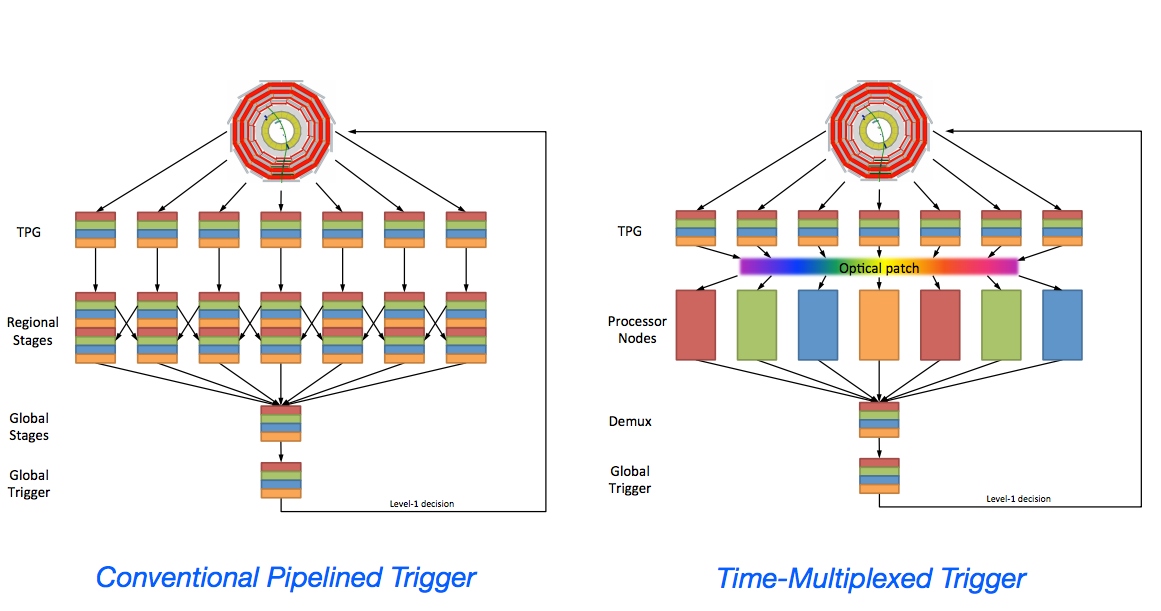
\includegraphics[width=0.9\textwidth]{./Figures/tmux}
  \caption{Comparison of the legacy and upgrade trigger systems where colour indicates the time slice \cite{JBrooke}. The TPG is the Trigger Primitive Generator from the ECAL and HCAL.}
  \label{tmux}
\end{figure}
